\documentclass{standalone}
\usepackage{tikz}
\usepackage{graphicx}
\usepackage[dvipsnames]{xcolor}
\usepackage{anyfontsize}

\definecolor{yell}{HTML}{ffde59}
\definecolor{oran}{HTML}{fb7e00}

\begin{document}
\begin{tikzpicture}[scale=1, transform shape]
	\node[anchor=south west] at (0, 0) {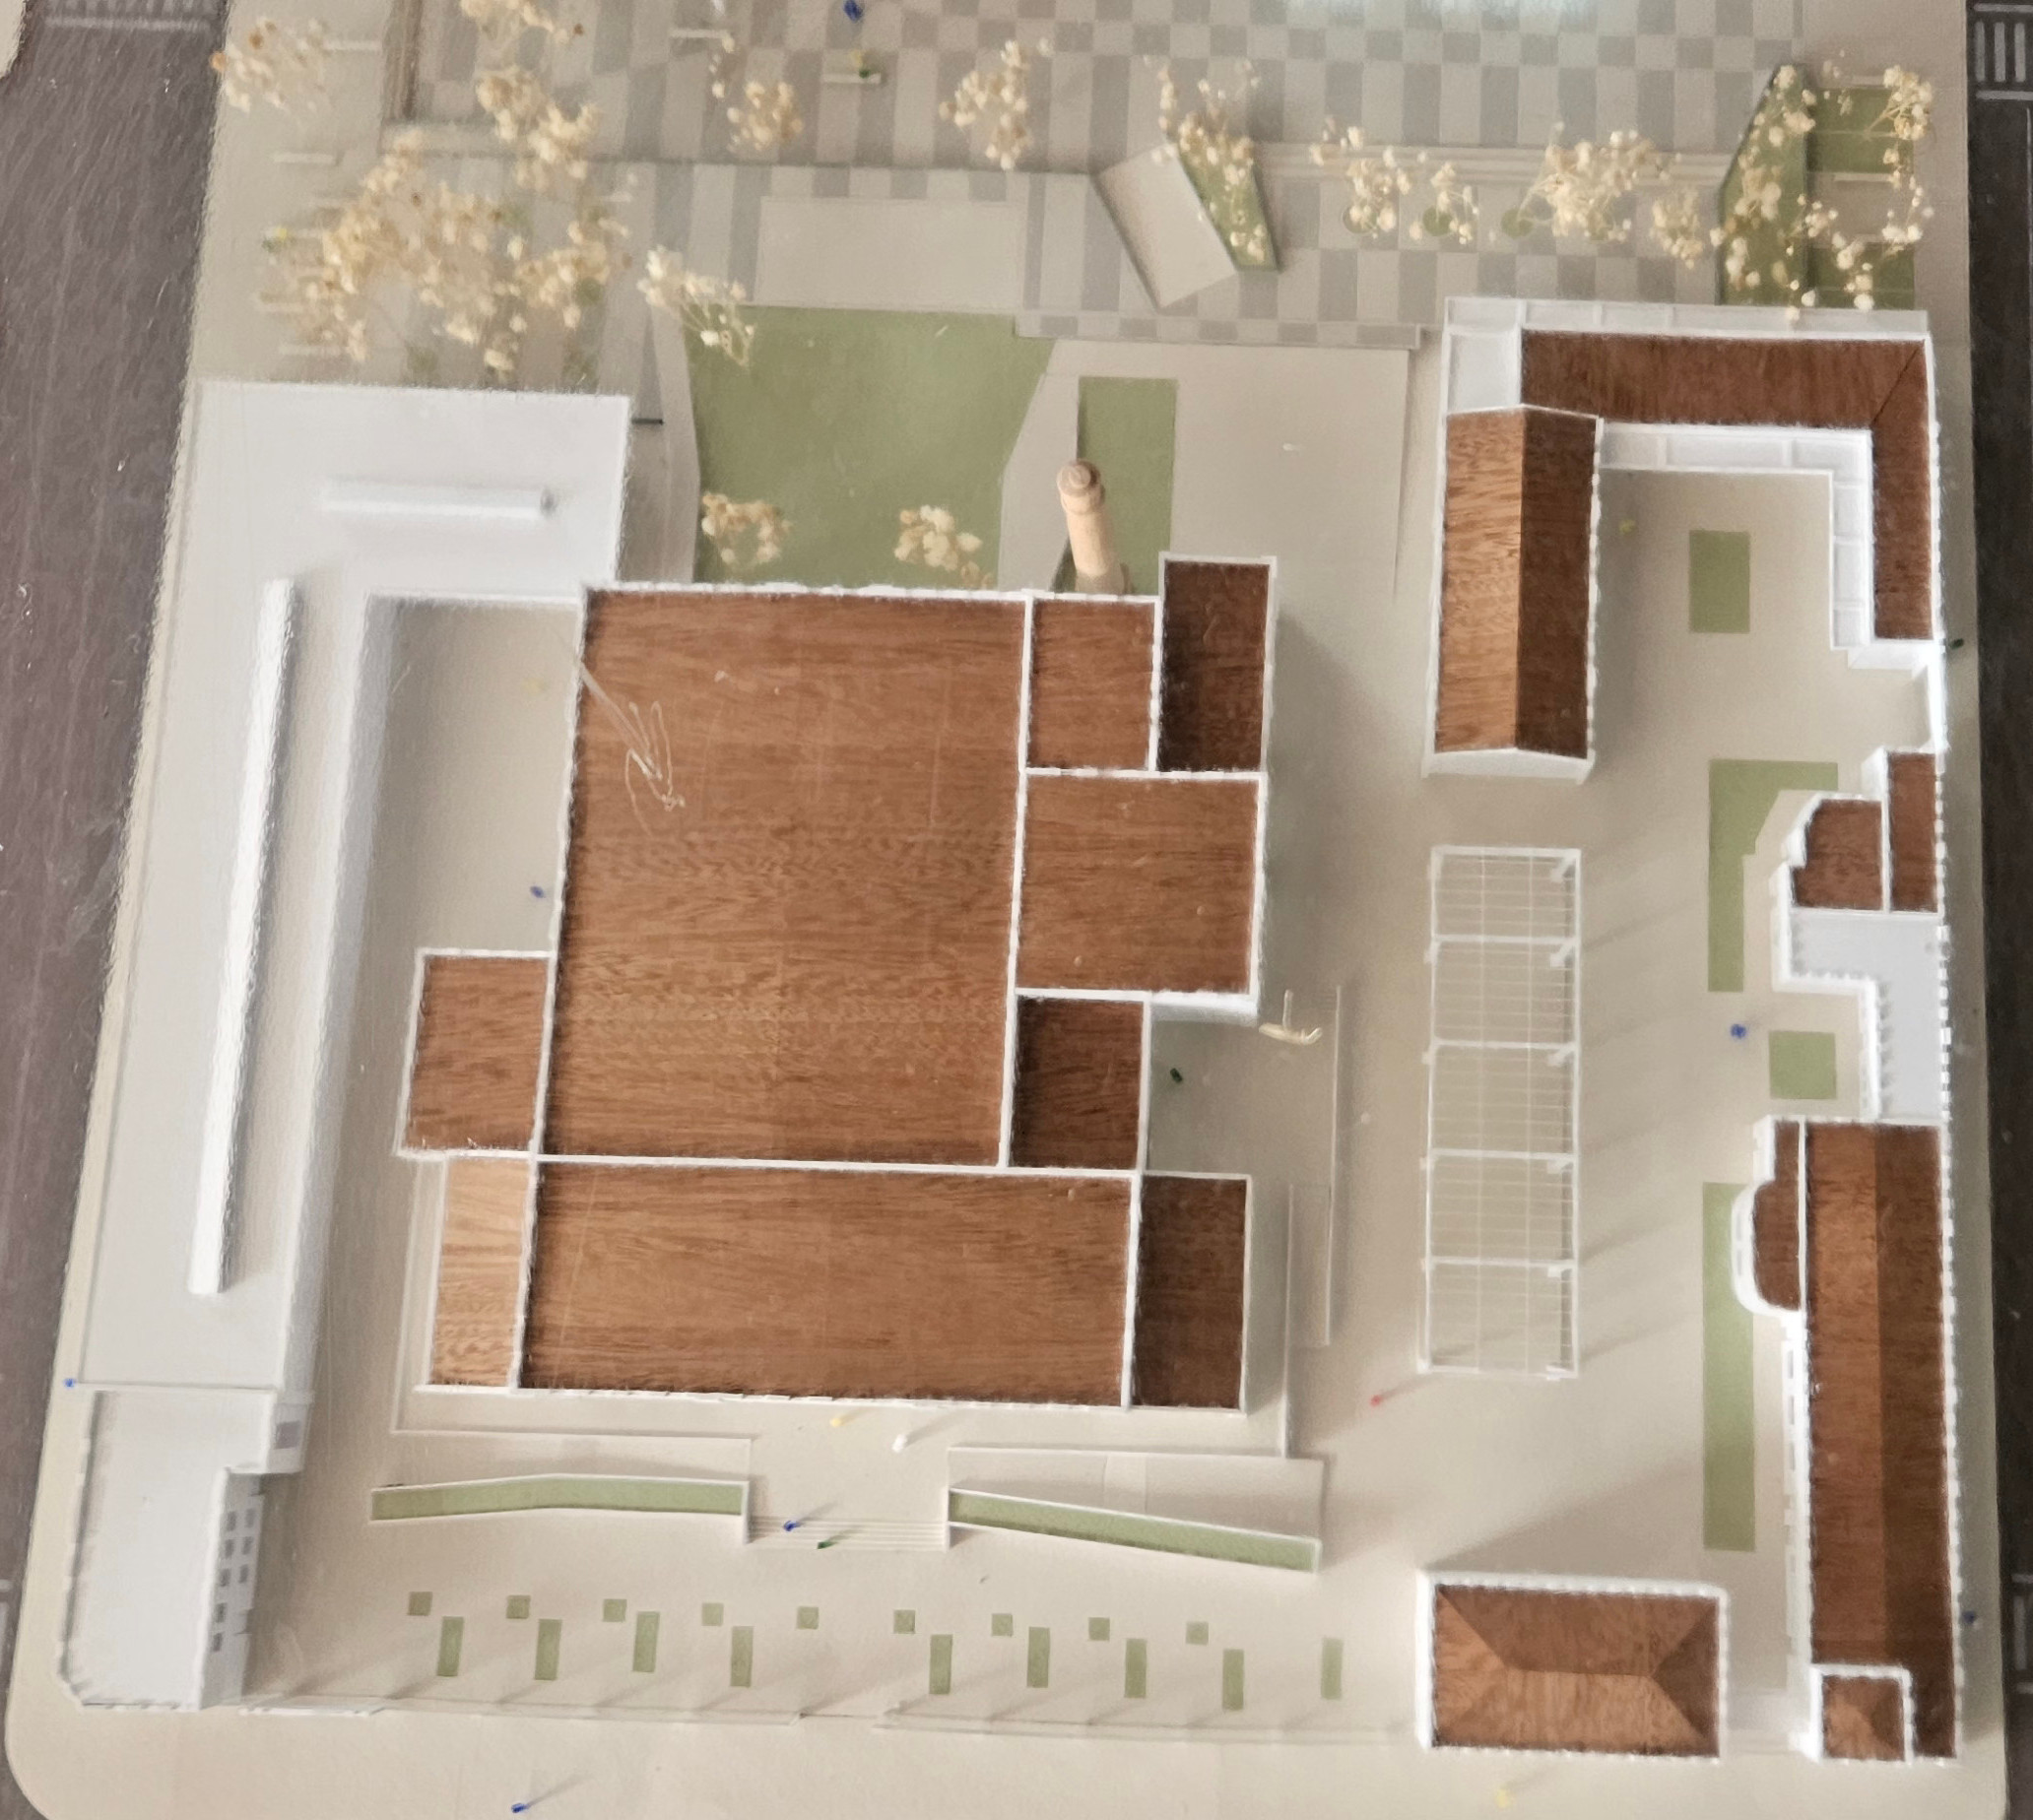
\includegraphics{../../Photos/model-02.jpg}};

	\node (Bib) at (21, 44.3) {};
	\draw[fill=yell, thin, nearly opaque] (Bib) -- ++(16.0, -0.3) -- ++(-1.0, -20.8)
		-- ++(-16.5, 0.8) -- cycle;
	\node[font=\fontsize{60}{12}\selectfont, below of=Bib, shift={(7.5,-9.7)}]
		{Biblioteca};

	\node (AudCent) at (36.9, 37.7) {};
	\draw[fill=oran, thin, nearly opaque] (AudCent) -- ++(8.6, -0.2) --
		++(-0.5, -8.0) -- ++(-8.5, 0.5) -- cycle;
	\node[font=\fontsize{60}{12}\selectfont, align=center, below of=AudCent,
		shift={(4.1,-3)}] {Aud. \\ Central};

	\node (Caldas) at (41.0, 23.3) {};
	\draw[fill=Plum, thin, nearly opaque] (Caldas) -- ++(3.8, -0.1) --
		++(-0.2, -8.4) -- ++(-4.0, 0.0) -- cycle;
	\node[font=\fontsize{60}{12}\selectfont, rotate=90, below of=Caldas,
		shift={(-4.0,-1.0)}] {Caldas};

	\node (Mutis) at (16.0, 24) {};
	\draw[fill=Green, thin, nearly opaque] (Mutis) -- ++(3.0, -0.1) --
		++(-0.5, -8.4) -- ++(-3.0, 0.1) -- cycle;
	\node[font=\fontsize{60}{12}\selectfont, rotate=90, below of=Mutis,
		shift={(-4.3, -0.1)}] {Mutis};

	\node (Palabra) at (51.5, 35) {};
	\draw[fill=Cyan, thin, nearly opaque] (Palabra) -- ++(5.0, -0.1) --
		++(0.0, -18.8) -- ++(-5.2, 0.1) -- cycle;
	\node[font=\fontsize{60}{12}\selectfont, rotate=90, below of=Palabra,
		shift={(-9.3, -1.5)}] {Plaza Palabra};

	\node (Cafe) at (57.0, 50) {};
	\draw[fill=Brown, thin, nearly opaque] (Cafe) -- ++(10.0, -0.1) --
		++(0.0, -11.0) -- ++(-10.0, 0.1) -- cycle;
	\node[font=\fontsize{60}{12}\selectfont, align=center, below of=Cafe,
		shift={(5.0, -4.5)}] {Plaza \\ Café};

	\node (AudInv) at (7.5, 51.7) {};
	\draw[fill=JungleGreen, thin, nearly opaque] (AudInv) -- ++(15.0, -0.3) --
		++(0.0, -7.0) -- ++(-16.0, 0.0) -- cycle;
	\node[font=\fontsize{60}{12}\selectfont, below of=AudInv,
		shift={(7.0, -2.5)}] {Audi. Invest.};

	\node (Invest) at (6.5, 44.5) {};
	\draw[fill=Red, thin, nearly opaque] (Invest) -- ++(7.0, -0.3) --
		++(-3.5, -30.0) -- ++(-7.0, 0.0) -- cycle;
	\node[font=\fontsize{60}{12}\selectfont, rotate=90, below of=Invest,
		shift={(-14.0, -1.0)}] {Investigadores};
\end{tikzpicture}
\end{document}
